\begin{frame}{What is Browser Fingerprinting}
  Browser Fingerprinting is a method that allows websites and online services to collect and analyze specific data about a user's device resulting in a unique fingerprint of it.
  \begin{figure}
    \centering
    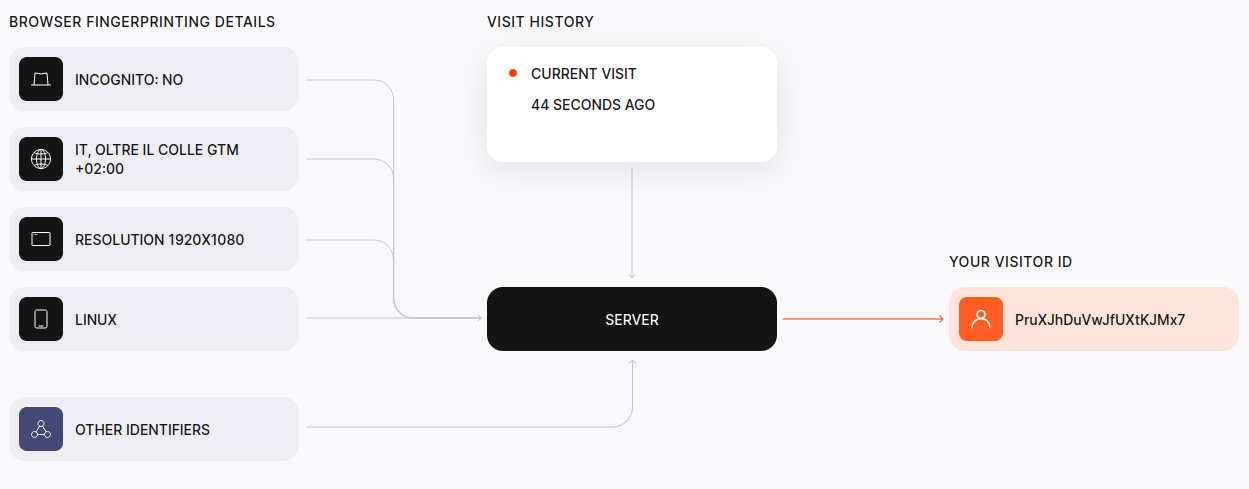
\includegraphics[width=\linewidth]{images/fingerprint.png}
  \end{figure}
\end{frame}

\begin{frame}{Which data is collected}
  \begin{itemize}
    \item \textbf{Browser info:} type, version, language, plugins, settings, \dots
    \item \textbf{Device info:} os, gpu, screen size, fonts, battery info, \dots
    \item \textbf{Network and Session info:} public ip, local ip, timezone, supported protocols and ciphers, \dots
  \end{itemize}
\end{frame}

\begin{frame}{Browser Fingerprinting properties: uniqueness}
  It is highly improbable for two users to have identical fingerprints.
  In fact, studies have suggested the uniqueness can be so specific that only one in several hundred thousand users might share the same fingerprint.

  \begin{figure}
    \centering
    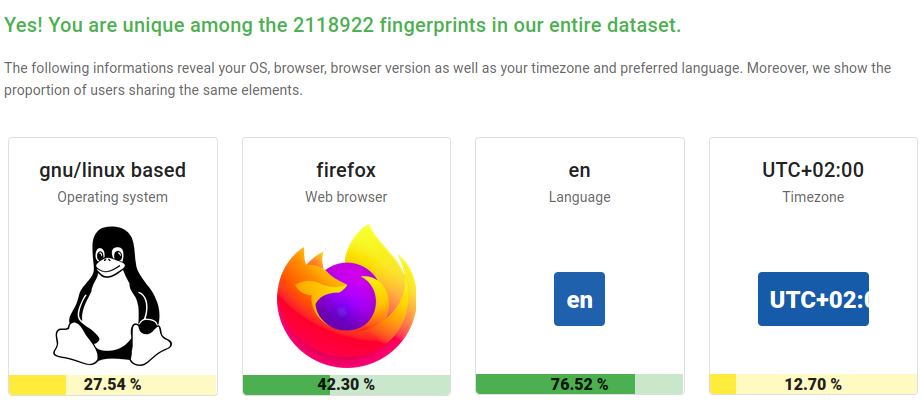
\includegraphics[width=\linewidth]{images/uniqueness.png}
  \end{figure}
\end{frame}

\begin{frame}{Browser Fingerprinting properties: stateless}
  Even if users disable cookies, change IP or use privacy-focused browsing modes, fingerprinting can still function, making it both challenging to detect and thwart.
  This method is stateless, not relying on stored data in the browser, and hence, it leaves no obvious trace.

  \begin{figure}
    \centering
    \begin{subfigure}{0.45\textwidth}
      
\includegraphics[width=\linewidth]{images/fingerprint-ip-1.png}
    \end{subfigure}
    \begin{subfigure}{0.45\textwidth}
      
\includegraphics[width=\linewidth]{images/fingerprint-ip-2.png}
    \end{subfigure}
  \end{figure}
\end{frame}